\section{Theta rhythmicity of saccades}\label{sec:theta_rhythmicity_of_saccades}
The approximate \qty{200}{\ms} timescale of human saccades has long existed experimentally \cite{meyer_rhythmicity_1966, saccadic_rhythm_1986, chota_rhythmic_2018, shaverdi_orchestration_2023}. A direct measure of saccade rhythmicity is the direct measurement of the spread of the ISI distribution, assuming a large lognormal spread of intervals $\Delta t$. This can be used to construct a measure called the Rhythmicity Index (RI):
\begin{equation}
	\text{RI} = \frac{1}{\text{CV}_{\ln}}, \qquad \text{CV}_{\ln} = \sqrt{e^{\sigma_{\ln}^2} - 1}
\end{equation}
where $\sigma_{\ln}$ is the standard deviation of the distribution of ISIs in log-space $\ln \Delta t$, with $\text{CV}_{\ln}$ often called the geometric CV. This $\text{RI}$ is an effective measure of the spread of a strictly positive distribution. A Poisson distributed variable will give $\text{RI}=1$, whereas it is found that for the ISI distribution of subjects considered here for a random NOISE condition is $\text{RI} = 2.69$ \cite{naher_primate_saccades}.

\subsection{Local rhythmicity of saccades}
The recent discovery of the strength of saccade rhythmicity by \textcite{naher_primate_saccades} and others \cite{zubair_eye_2026} required a deep understanding of the rhythmicity of biological systems. A challenge that is often present in biological systems is that timescales are not driven by a perfect clock, but instead the characteristic timescales of certain regular patterns in the brain. As such, the \qty{200}{\milli \second} estimate for saccades during a visual search is not expected to be a universal timescale across subjects and trials. Instead, the model used for such processes in neuroscientific works is a noisy rise-to-threshold model, where a random walk is constructed, and when it reaches a goal, a decision is made \cite{naher_primate_saccades} [CITE]. The noise-driven rise for this process is expected to have a rate which is slowly varying about a characteristic timescale, in the case of saccades around \qtyrange{2}{6}{\hertz}. Since this slowly varying rate is expected to be stable for a single individual and a single trial, we consider a local measure of rhythmicity for the intervals between the saccades within a timseries, called the Inter-Saccadic-Intervals (ISI). Such a metric can be proposed---as developed by \cite{naher_primate_saccades}---with the local Rate-Corrected Rhythmicity Index (RCRI):
\begin{equation}\label{eq:RCRI}
	\text{RCRI} = \frac{1}{1 + \langle \text{CV}_2 \rangle}, \qquad \text{CV}_2(i) = 2\frac{\|\Delta t_{i+1} - \Delta t_{i} \|}{\Delta t_{i+1} + \Delta t_{i}}
\end{equation}
which allows quantification of purely local rhythmicity, comparing each interval $\Delta t_{i+1}$ to it's predecessor $\Delta t_{i}$, and averaging across all intervals considered $i$, usually a single subject. The results of such an analysis have resulted in two key conclusions. Firstly, human saccades are very strongly rhythmic, with $\text{RCRI}\approx0.76$ for the subjects as described in \cref{sec:model_setup} depending on condition. Secondly, it has been found that the instantaneous saccade rate is a strong predictor for the local saccade rhythmicity $\text{RCRI}$, with a correlation calculated at $\rho=0.39, P=0.001$, with saccade rate found to be a significant predictor of $\text{RCRI}$ with $\beta=\qty{0.0114}{\hertz^{-1}}, P=0.014$

those particular individuals and trials binned with a higher saccade rate correlate with higher RCRI and thus stronger comparable rhythmicity \cite{naher_primate_saccades}, as shown in \cref{fig:rate-RCRI}.
\begin{figure}[htbp]
	\centering
	\begin{subfigure}[T]{0.45\textwidth}
		\centering
		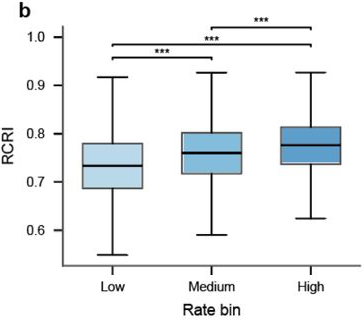
\includegraphics[width=\linewidth]{figures/RCRI.png}
		\caption{\textbf{Rate-corrected rhythmicity index (RCRI) is positively correlated with saccade rate.} Collaborators \textcite{naher_primate_saccades} uncovered this statistically significant result, which implies that shorter inter-saccadic intervals (ISIs) will result in more regular ISIs, which corresponds to stronger kernel dynamics as defined in \cref{subsec:adaptive_kernel_dynamics}.}
		\label{fig:rate-RCRI}
	\end{subfigure}
	\hfill
	\begin{subfigure}[T]{0.45\textwidth}
		\centering
		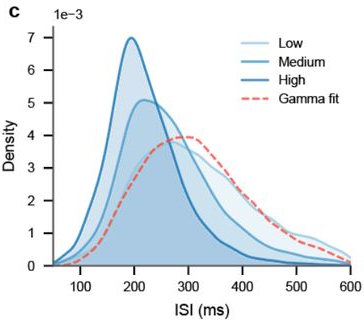
\includegraphics[width=\linewidth]{figures/ISI.png}
		\caption{\textbf{The probability distribution of inter-saccadic intervals (ISIs) are tightly distributed in a Gamma-10 distribution.} Our collaborators in \textcite{naher_primate_saccades} find that saccades are more locally rhythmic than previously considered. In particular, the ISI distribution is a tight Gamma-10 distribution, but the ISI timeseries is strongly locally rhythmic, as captured by the rate-corrected rhythmicity index (RCRI).}
		\label{fig:gamma_fits}
	\end{subfigure}
	\caption{}
	\label{fig:local_rhythmicity}
\end{figure}
\subsubsection*{Interpretations of local rhythmicity and saccade rate for a model of gaze dynamics}
These results support our unified stochastic-informative formulation of gaze dynamics. We have shown good agreement between the tight distribution of modelled ISIs, more closely locally. We have also introduced a natural parameter $\tau$ with which to modulate the slowly varying theta-scale saccade rate. This also connects the dynamics of information gathering with the dynamics of regular attention in a search task. The results that rhythmicity is strongest where a task contains nearly identical searched objects is encouraging for this information-driven saccade rate theory. A correlation between high saccade rate and high rhythmicity is predicted from the origin of regular dynamical-informational transitions as described in \cref{sec:dynamical-information_adaptation}, where a stronger kernel produces more rhythmic transitions, and a weaker kernel will approach an arrhythmic Poisson point distribution of ISIs, reducing the RCRI, as predicted.